\section{Data Samples and Event Selection}

Trigger, DataSample, Good Run List. Mention separate 900 GeV and 2.36
TeV. 

\subsection{Vertex selection}
Show vertex distributions, discuss some group's selections on vertex.

\subsection{Removal of scraping events}
This is an example of subsection

\subsection{HCAL anomalous noise}

This is an example of subsection

\subsection{ECAL anomalous noise}

This is an example of subsection

\begin{2figures}{hbtp}
  \resizebox{8cm}{!}{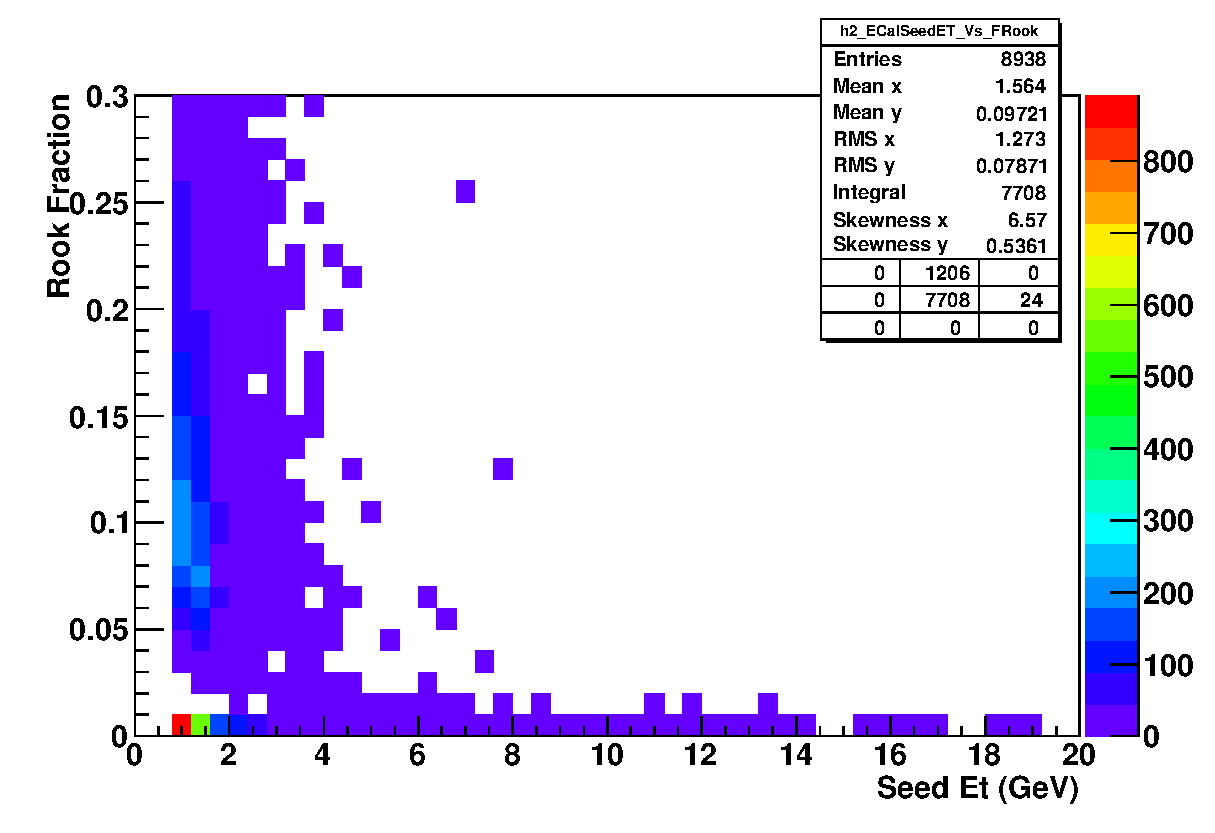
\includegraphics{plots_ecalnoise/SeedET_Frook_DATA900GeV.eps}} &
  \resizebox{8cm}{!}{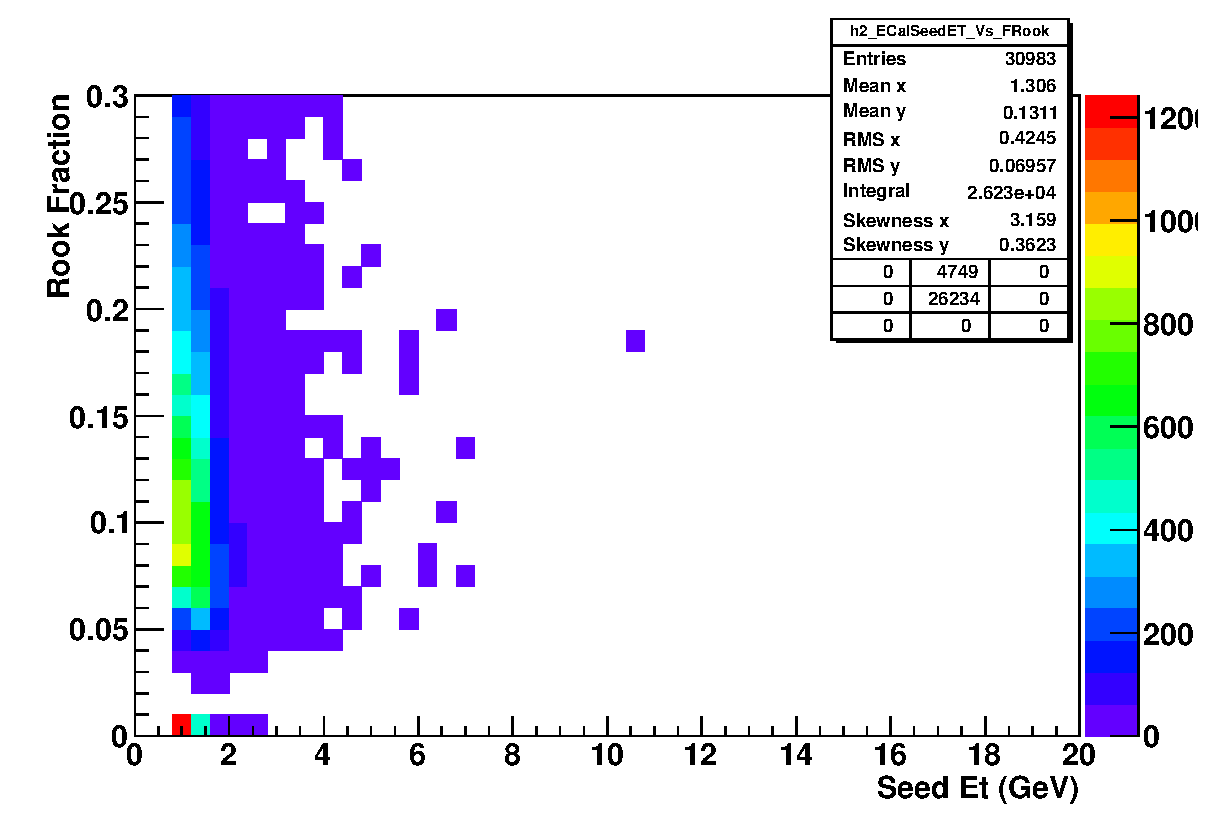
\includegraphics{plots_ecalnoise/SeedET_Frook_MC900GeV.eps}} \\
\caption{900 GeV Data Vs MC}
 \label{fig:ecal_noise_1}
\end{2figures}

Add cut efficiency table HERE.

\begin{table}[htbp]
 \label{tab:HEEPselection}
 \begin{center}
   \begin{tabular}{|lcc|lcc|} \hline
     \multicolumn{3}{|c|}{ID Variables} & \multicolumn{3}{|c|}{Isolation Variables} \\
     Variable & Barrel & Endcap & Variable & Barrel & Endcap  \\ \hline
     $H/E$  & $<0.05$ & $<0.1$ & $N_T$  & $<4$ & $<4$ \\ \hline
     $\sigma_{\eta\eta}$  & $<0.011$ & $<0.0275$ & Track iso (GeV) & $<7.5$ & $<15$ \\ \hline
     $|\Delta\eta^{trk-SC}|$ & $<0.005$ & $<0.007$ & EM iso (GeV) & $<6+0.01*E_{t}$ & $<6+0.01*E_{t}$ \\ \hline
     $|\Delta\phi^{trk-SC}|$ & $<0.09$ & $<0.09$ & HAD iso (GeV) & $<4+0.005*E_{t}$ & $<4+0.005*E_{t}$ \\ \hline
   \end{tabular}
 \caption{\small \sl HEEP electron ID and isolation criteria.
   Reconstructed electrons are associated to the
   barrel (endcaps) if $|\eta|<1.442$ ($1.560<|\eta|<2.5$).}
 \end{center}
\end{table}


\subsection{Effect of noise removal}
Here we put the $\etmiss$ distribution with base selection, after HCAL/ECAL
noise removal.
